\documentclass[12pt]{beamer}
\setbeamertemplate{navigation symbols}{}
%\usepackage[latin1]{inputenc}
\usepackage{pgfplots}
\usepackage{adjustbox}
\usepackage{graphicx}
%\usepackage{draftwatermark}
\usepackage{tikz}
\usepackage{colortbl}
\usepackage{subfigure}
%\usetheme{Amsterdam}
\usecolortheme{default}
\title[]{Government websites as data: A methodological pipeline for
collection, processing, and text analysis}
\author{Markus Neumann \\ Fridolin Linder \\ Bruce Desmarais}
\institute{The Pennsylvania State University}
\date{January 6, 2018}

\makeatletter
\defbeamertemplate*{footline}{myminiframes theme}
{%
	\begin{beamercolorbox}[colsep=1.5pt]{upper separation line foot}
	\end{beamercolorbox}
	\hbox{%
		\begin{beamercolorbox}[wd=.1\paperwidth,ht=2.5ex,dp=1.125ex,%
			leftskip=.3cm,rightskip=.3cm,center]{title in head/foot}%
			{\usebeamerfont{author in head/foot}\usebeamercolor[fg]{author in head/foot}}{\insertframenumber}%/\inserttotalframenumber}%
		\end{beamercolorbox}%
		\begin{beamercolorbox}[wd=.75\paperwidth,ht=2.5ex,dp=1.125ex,%
			leftskip=.3cm,rightskip=.3cm plus1fil,center]{title in head/foot}%
			\leavevmode{\usebeamerfont{title in head/foot}\insertshorttitle}%
		\end{beamercolorbox}%
		\begin{beamercolorbox}[wd=.15\paperwidth,ht=2.5ex,dp=1.125ex,%
			leftskip=.3cm,rightskip=.3cm plus1fil,center]{title in head/foot}%
			{\usebeamerfont{author in head/foot}\usebeamercolor[fg]{author in head/foot}}%\insertshortauthor}
		\end{beamercolorbox}%
	}%
	\begin{beamercolorbox}[colsep=1.5pt]{lower separation line foot}
	\end{beamercolorbox}
}
\makeatother

\begin{document}

\section{Introduction}
\begin{frame}
\titlepage
\end{frame}

\begin{frame}{Presented at SPSA}
	\textbf{Data Collection} \hspace{2mm} $\rightarrow$ \hspace{2mm} \textbf{Preprocessing} \hspace{2mm} $\rightarrow$ \hspace{2mm} \textbf{Analysis}
\begin{columns}
	\column{0.33\textwidth}
	%Data Collection
	\vspace{5mm}
	\begin{itemize}
		\item Identify URLs
		\item Verify URLs (browser automation)
		\item Download websites
		\item Determine file type
		\item Convert to txt
	\end{itemize}		
	\column{0.33\textwidth}
	%Preprocessing
	\vspace{5mm}
	\begin{itemize}
		\item Remove punctuation, dates, etc.
		\item To lowercase
		\item Boilerplate removal
		\item Spellchecking
		\item Lemmatization \\ (city \& cities = city)
	\end{itemize}
	\column{0.33\textwidth}
	%Analysis
	\vspace{5mm}
	\begin{itemize}
		%\item Hierarchical clustering
		\item Fightin' Words
		\item Structural topic model
		%\begin{itemize}
		%	\item LDA
		%	\item STM
		%\end{itemize}
	\end{itemize}
\end{columns}
\end{frame}

\begin{frame}{Presented at SPSA}
% latex table generated in R 3.4.2 by xtable 1.8-2 package
% Wed Dec 27 19:51:57 2017
\begin{table}[ht]
\centering
\begin{tabular}{rrrr}
  \hline
 & Democratic & Republican & Total \\ 
  \hline
Cities & 16 & 17 & 33 \\ 
  Documents & 10868 & 6438 & 17306 \\ 
  Token types & 20774 & 17947 & 21697 \\ 
  Token instances & 6532383 & 2651876 & 9184259 \\ 
   \hline
\end{tabular}
\caption{Indiana} 
\end{table}


% latex table generated in R 3.4.2 by xtable 1.8-2 package
% Wed Dec 27 19:55:34 2017
\begin{table}[ht]
\centering
\begin{tabular}{rrrr}
  \hline
 & Democratic & Republican & Total \\ 
  \hline
Cities & 10 & 8 & 18 \\ 
  Documents & 6636 & 1378 & 8014 \\ 
  Token types & 16649 & 9234 & 16856 \\ 
  Token instances & 3764877 & 355774 & 4120651 \\ 
   \hline
\end{tabular}
\caption{Louisiana} 
\end{table}


\end{frame}

\begin{frame}{Presented at SPSA}
\begin{figure}
	\hfill
	\subfigure{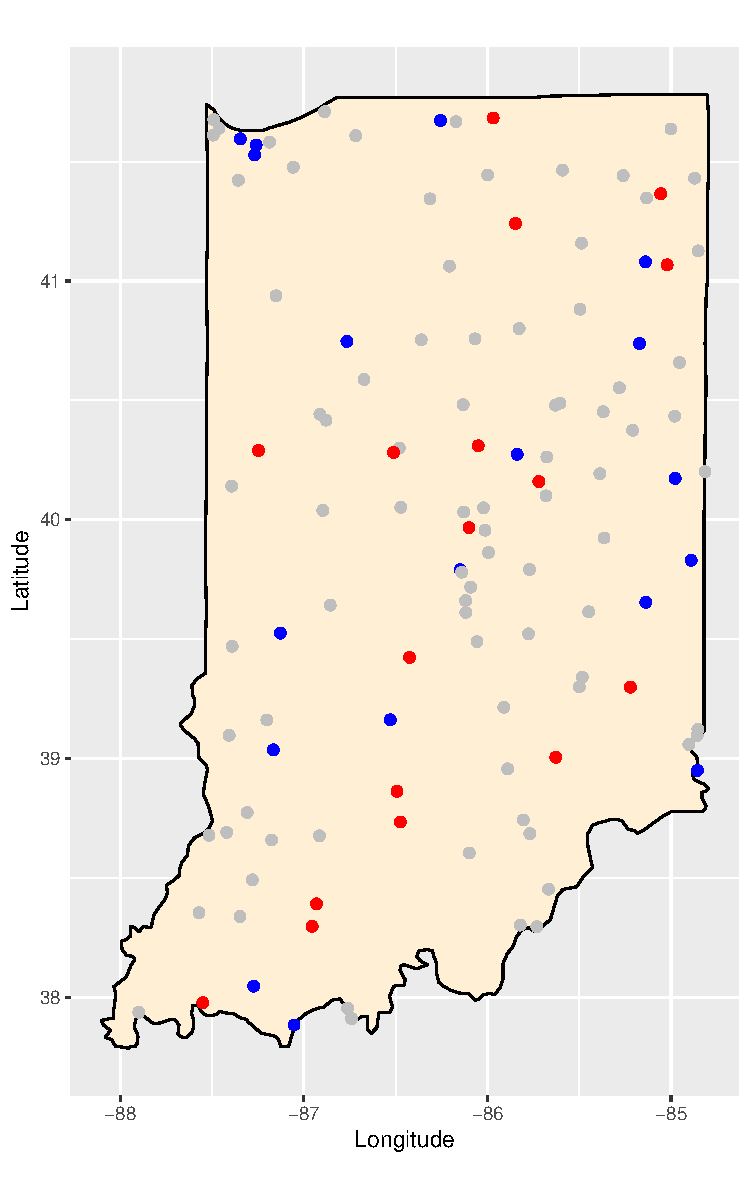
\includegraphics[width=5cm, height = .7\textheight]{../figures/indiana_map.pdf}}
	\hfill
	\subfigure{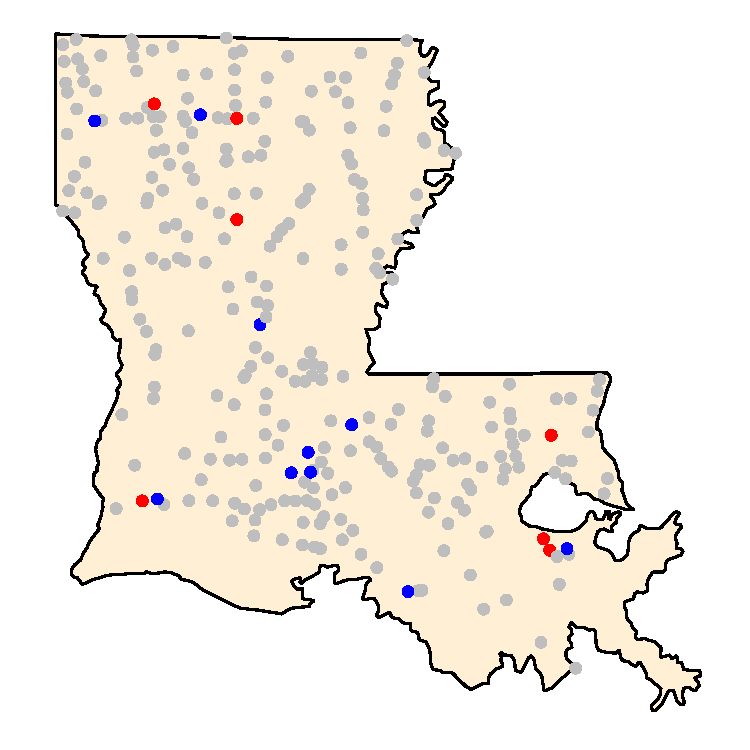
\includegraphics[width=5cm, height = .7\textheight]{../figures/louisiana_map.pdf}}
\end{figure}
\end{frame}

\begin{frame}{Presented at SPSA}
	% latex table generated in R 3.4.1 by xtable 1.8-2 package
% Fri Oct 20 10:49:17 2017
\begin{table}[ht]
\centering
\begingroup\fontsize{9pt}{10pt}\selectfont
\begin{tabular}{lrlr}
  \hline
Word (D) & z-Score (D) & Word (R) & z-Score (R) \\ 
  \hline
said & 86.20 & request & 69.41 \\ 
  proposal & 70.98 & member & 67.45 \\ 
  fund & 59.22 & street & 47.84 \\ 
  county & 54.15 & motion & 46.35 \\ 
  asked & 52.62 & councilor & 45.69 \\ 
  budget & 49.40 & main & 44.34 \\ 
  stated & 46.90 & goods & 44.33 \\ 
  tax & 41.79 & use & 43.43 \\ 
  fort & 41.17 & tree & 42.77 \\ 
  ms & 40.76 & amp & 42.48 \\ 
  division & 38.01 & water & 41.45 \\ 
  million & 36.62 & downtown & 40.66 \\ 
  grants & 35.21 & pm & 39.60 \\ 
  introduced & 34.85 & sign & 39.28 \\ 
  contract & 34.36 & st & 38.23 \\ 
  revenue & 34.33 & plan & 38.20 \\ 
  general & 34.17 & rd & 37.71 \\ 
  chair & 32.01 & site & 37.19 \\ 
  brown & 31.86 & docket & 37.03 \\ 
  federal & 31.46 & trees & 36.56 \\ 
  metropolitan & 31.25 & plat & 36.15 \\ 
  management & 30.69 & old & 35.44 \\ 
  agency & 30.35 & residential & 34.65 \\ 
  approves & 29.66 & area & 34.31 \\ 
  authorizes & 29.11 & variance & 33.50 \\ 
  technology & 28.45 & th & 33.20 \\ 
  provide & 27.43 & utility & 33.11 \\ 
  dollars & 27.30 & ordinance & 32.04 \\ 
  consolidated & 26.29 & carter & 31.40 \\ 
  justice & 25.93 & approve & 31.40 \\ 
  parks & 25.79 & building & 30.78 \\ 
  lewis & 25.73 & feet & 30.16 \\ 
  increase & 25.66 & news & 29.37 \\ 
  digest & 25.60 & city & 29.26 \\ 
  support & 25.43 & lots & 29.19 \\ 
  oliver & 25.43 & lot & 28.89 \\ 
  animal & 25.02 & aid & 28.54 \\ 
  gray & 24.72 & overlay & 28.53 \\ 
  capital & 24.54 & home & 28.52 \\ 
  services & 24.53 & democrat & 28.40 \\ 
  amends & 23.84 & republican & 28.25 \\ 
  criminal & 23.70 & uses & 28.05 \\ 
  enterprise & 23.62 & must & 27.57 \\ 
  mayors & 23.51 & legal & 26.64 \\ 
  court & 22.90 & zoning & 26.53 \\ 
  township & 22.86 & councilors & 26.50 \\ 
  controls & 22.54 & river & 26.48 \\ 
  funded & 22.28 & stellar & 26.40 \\ 
  referred & 22.16 & common & 26.15 \\ 
  fiscal & 22.10 & rep & 26.03 \\ 
   \hline
\end{tabular}
\endgroup
\caption{Top 50 democratic and Republican words (Indiana), according to the informed 
             Dirichlet model of Monroe et al. (2008).} 
\label{tabFightinIN}
\end{table}


\end{frame}

\begin{frame}{Presented at SPSA}
% latex table generated in R 3.4.3 by xtable 1.8-2 package
% Tue Dec 26 20:59:22 2017
\begin{table}[ht]
\centering
\scriptsize
\begin{tabular}{llllll}
  \hline
-0.027 & -0.022 & -0.016 & -0.011 & -0.011 & -0.01 \\ 
  \hline
city & school & downtown & city & \cellcolor{blue!25}trash & \cellcolor{blue!25}housing \\ 
  ordinance & community & business & department & city & property \\ 
  approve & program & project & mayor & \cellcolor{blue!25}waste & program \\ 
  resolution & student & city & police & day & \cellcolor{blue!25}fund \\ 
  property & \cellcolor{blue!25}education & \cellcolor{blue!25}development & officer & \cellcolor{blue!25}recycle & home \\ 
  purchase & \cellcolor{blue!25}university & new & public & street & city \\ 
  area & national & center & citizen & collection & project \\ 
  department & award & \cellcolor{blue!25}economic & work & resident & neighborhood \\ 
  contract & high & company & safety & \cellcolor{blue!25}recycling & \cellcolor{blue!25}grant \\ 
  service & year & community & resident & snow & unit \\ 
   \hline
\end{tabular}
\caption{Top Democratic topics and words}%\caption{Top Democratic topics and words (Indiana), according to STM. 
%The words are the top words for the most Democratic/Republican topic, determined
%by the size (and significance) of the coefficient (see table header) of the party covariate.} 
\label{tabSTMINDem}
\end{table}

 %../tables/stmTopWordsINDem.tex
\end{frame}

\begin{frame}{Presented at SPSA}
% latex table generated in R 3.4.2 by xtable 1.8-2 package
% Mon Nov 13 15:36:58 2017
\begin{table}[ht]
\centering
\begin{tabular}{llllll}
  \hline
0.024 & 0.019 & 0.019 & 0.016 & 0.016 & 0.016 \\ 
  \hline
motion & plan & inc & request & council & \cellcolor{red!25} traffic \\ 
  second & \cellcolor{red!25} zone & electr & board & citi & amp \\ 
  made & applic & build & member & ordin & vehicl \\ 
  approv & \cellcolor{red!25} properti & construct & servic & common & stop \\ 
  mayor & approv & home & \cellcolor{red!25} street & councilor & sign \\ 
  present & sign & street & approv & amend & \cellcolor{red!25} road \\ 
  state & \cellcolor{red!25} site & meridian & purchas & resolut & block \\ 
  will & locat & servic & citi & adopt & signal \\ 
  citi & commiss & west & move & wherea & \cellcolor{red!25} street \\ 
  council & file & main & good & approv & driver \\ 
   \hline
\end{tabular}
%\caption{Top Republican topics and words (Indiana), according to STM. 
%The words are the top words for the most Democratic/Republican topic, determined
%by the size (and significance) of the coefficient (see table header) of the party covariate.} 
\label{tabSTMINRep}
\end{table}

 %../tables/stmTopWordsINRep.tex
\end{frame}

\begin{frame}{SPSA feedback}
\begin{itemize}
	\item overall quite positive
	\item there seems to be some demand in publican administration for this kind of research
	\item threshold of ten for duplicates
	\item the usual concerns with bag-of-words
	\item describe methods more clearly
	\item \textbf{``Does your method improve the external validity so greatly that the internal validity becomes less of a concern?''}
	\item comparison with non-partisan cities/websites
	\item city covariates
\end{itemize}
\end{frame}

\begin{frame}{Planned covariates}
\begin{itemize}
	\item population
	\item GDP per capita
	\item percent non-white
	\item City area
	\item democratic vote share/magnitude of victory
	\item log median house price
	\item (most of these are from Einstein \& Glick 2015)
\end{itemize}
\end{frame}

\begin{frame}{Since SPSA - ground truth test}
\begin{itemize}
	\item party manifestos (didn't work - not enough data)
	\item mayors' campaign websites (LA/IN - didn't work - not much data, and strange results)
	\item mayors' campaign websites (top 100 cities - worked somewhat)
\end{itemize}
{\renewcommand\normalsize{\tiny}%
	\small
	% latex table generated in R 3.4.3 by xtable 1.8-2 package
% Tue Feb 13 10:36:40 2018
\begin{table}[ht]
\centering
\begin{tabular}{rllll}
  \hline
 & dem.groundtruth & rep.groundtruth & dem.cities & rep.cities \\ 
  \hline
dem.groundtruth & 1, 1 & 0.807, 0.896 & 0.714, 0.729 & 0.68, 0.698 \\ 
  rep.groundtruth & 0.807, 0.896 & 1, 1 & 0.647, 0.697 & 0.641, 0.693 \\ 
  dem.cities & 0.714, 0.729 & 0.647, 0.697 & 1, 1 & 0.937, 0.944 \\ 
  rep.cities & 0.68, 0.698 & 0.641, 0.693 & 0.937, 0.944 & 1, 1 \\ 
   \hline
\end{tabular}
\caption{Ground truth test, comparing campaign websites of mayors of the 100 largest cities in the US and cities in Indiana and Louisiana. The values are bootstrapped confidence bounds for cosine similarities between concatenated document collections.} 
\label{groundtruth_bootstrapped}
\end{table}

}
\end{frame}

\begin{frame}{Since SPSA - extending the sample}
\begin{itemize}
	\item New York
	\item big cities
	\item Washington
	\item Oregon (unsuccessful)
	\item extended LA/IN (55 -> 165)
	\item 314 cities total, 230 downloaded so far
\end{itemize}
\end{frame}

\begin{frame}{wget and www}
\begin{itemize}
	\item www.townoflockport.com/ -- doesn't work
	\item http://townoflockport.com/ -- works
	\item inconsistent across websites
	\item solution: check every website with Selenium, record the url it redirects to
	\item currently re-scraping the 84 websites still missing
\end{itemize}
\end{frame}

\begin{frame}{Next steps: compression}
\begin{itemize}
	\item Since, so far, something has always gone wrong when adjusting file endings and converting files to text, I've always made zipped backups so far
	\item compression of millions of files of more than 1TB
	\begin{itemize}
		\item time
		\item some paths are too long
		\item some filenames have non-ascii characters
	\end{itemize}
\end{itemize}
\end{frame}

\begin{frame}{Next steps: map}
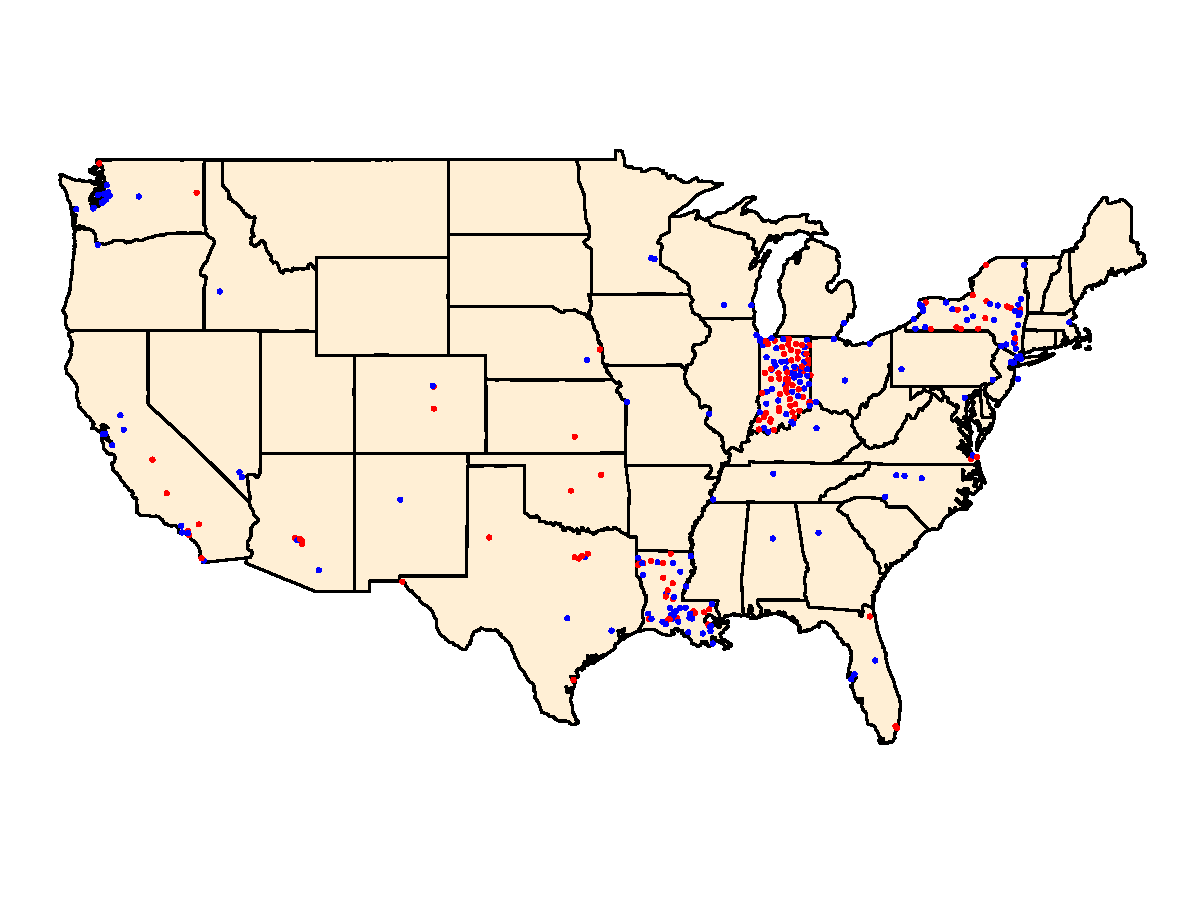
\includegraphics[width=\linewidth, height = .99\textheight]{../figures/us_map.pdf}
\end{frame}

\begin{frame}{Next steps: covariates}
\begin{itemize}
	\item I already downloaded the above some time ago, but only for LA and IN
	\item this was already a little convoluted, I'll have to automate it for it to work with all states
	\item there is a problem with the census data:
\end{itemize}
\end{frame}

\begin{frame}{Next steps: covariates}
\begin{itemize}
	\item I already downloaded the above some time ago, but only for LA and IN
	\item this was already a little convoluted, I'll have to automate it for it to work with all states
	\item there is a problem with the census data:
\end{itemize}
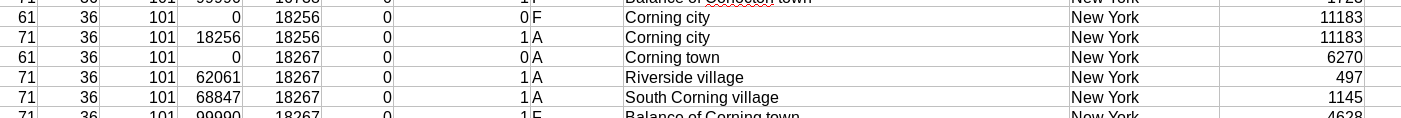
\includegraphics[width=\linewidth]{census_problem.png}
\begin{itemize}
	\item Not a priority right now, need to finish all the document-related stuff first
\end{itemize}
\end{frame}

\begin{frame}{Next steps: optimize code}
\begin{itemize}
	\item preprocessing already took 4-5 hours for 25000 documents
	\item we currently have 1.3 million; this will get reduced a bit, but it will still be a huge increase
	\item the functions that aren't already vectorized are currently ``sapply'd''
	\item with this much data, parallelization is probably worth it (currently only hashtables, spellchecking and some other more computationally intensive stuff is parallelized)
	\item MAYBE it would be worth it to translate everything to quanteda - but unfortunately that won't work with the hashtables stuff
	\item fightin' words is pretty fast, but stm also took hours already
\end{itemize}
\end{frame}

\begin{frame}{Next steps: structural topic model}
\begin{itemize}
	\item currently we use separate models for IN, LA
	\item state fixed effects
	\item package has problems with overly complex models
	\item maybe use stm only for IN, LA, NY, WA, CA
\end{itemize}
\end{frame}

\begin{frame}{STM Democratic}
% latex table generated in R 3.4.3 by xtable 1.8-2 package
% Tue Mar 20 09:25:03 2018
\begin{table}[ht]
\centering
\begingroup\tiny
\begin{tabular}{llllllll}
  \hline
-0.036 & -0.024 & -0.024 & -0.012 & -0.009 & -0.008 & -0.008 & -0.007 \\ 
  \hline
provide & applicant & community & council & department & shall & business & day \\ 
  otherwise & owner & city & councilman & division & city & development & contract \\ 
  city & application & neighborhood & rise & service & contractor & economic & total \\ 
  respect & new & public & mayor & police & agreement & downtown & payment \\ 
  authorize & building & mayor & city & city & person & job & invoice \\ 
  ordinance & exist & work & state & provide & provide & new & process \\ 
  thereto & proposal & program & grant & public & upon & city & department \\ 
  councilman & retention & resident & street & management & term & project & approval \\ 
  district & per & effort & fund & operation & provision & center & complete \\ 
  property & build & new & discussion & office & time & service & procurement \\ 
   \hline
\end{tabular}
\endgroup
\caption{Republican} 
\label{tabSTMIN_LADem}
\end{table}


\end{frame}

\begin{frame}{STM Republican}
% latex table generated in R 3.4.3 by xtable 1.8-2 package
% Tue Mar 20 09:25:03 2018
\begin{table}[ht]
\centering
\begingroup\tiny
\begin{tabular}{llllllll}
  \hline
0.019 & 0.018 & 0.016 & 0.015 & 0.015 & 0.013 & 0.012 & 0.01 \\ 
  \hline
library & park & motion & inc & proposal & say & lot & city \\ 
  stream & recreation & second & cross & digest & ask & district & information \\ 
  length & pool & make & construction & fund & state & use & day \\ 
  obj & facility & present & drive & grant & proposal & foot & contact \\ 
  pdf & center & approve & street & county & make & zone & can \\ 
  type & program & state & creek & authorize & get & street & resident \\ 
  branch & golf & minute & park & introduce & can & square & please \\ 
  unknown & playground & meeting & hill & district & need & area & department \\ 
  flag & trail & pass & ave & public & go & building & call \\ 
  image & play & mayor & oak & department & work & parking & amp \\ 
   \hline
\end{tabular}
\endgroup
\caption{Democratic} 
\label{tabSTMIN_LARep}
\end{table}


\end{frame}

\end{document}